
\subsection{Ejercicio A}
Realizamos una heurística golosa para resolver el problema. Lo que hace el algoritmo es lo siguiente. Primero toma los datos de entrada del problema, y se arma la matriz o las listas de adyacencia del grafo (según la implementación elegida). Además, se crea un vector de nodos de tamaño $n$ donde cada nodo contiene guardado su número de nodo y el grado que tiene en el grafo. \\ 
Una vez que se procesaron los datos de entrada, se procede a resolver el problema. Para esto, se ordena el arreglo de nodos según sus grados de mayor a menor. Luego, se crea un arreglo de booleanos de tamaño n, donde cada uno está inicializado en $false$. En este arreglo se guarda si el nodo ya fue visitado o no. También se crea un arreglo llamado $cidm$ donde se guardará la solución. \\ 
Por último, se recorre en orden el arreglo de nodos ordenados según su grado. Si un nodo no fue visitado, se agrega el nodo a $cidm$ y luego se marcan como visitados a todos sus adyacentes (ya que queremos que sea dominante y mínimo).
Una vez que se recorre todo el arreglo, ya tenemos el $cidm$, solo resta mostrarlo por pantalla.

\subsection{Pseudocódigo}

\subsubsection{Implementación sobre listas de adyacencia}
\begin{codesnippet}
Crear listas de adyacencia con el input
Crear arreglo nodos que guarda numero de nodo y grado para cada nodo

Ordenar arreglo nodos segun su grado
Crear vector de booleanos visitado de tamano n para guardar nodos visitados
Crear vector cidm para guardar la solucion

Para cada nodo u en el arreglo ordenado:
	Si el nodo no fue visitado:
		agregar el nodo a cidm
		Para cada nodo w en su lista de adyacencia:
			marcar w como visitado
		fin Para
	fin Si
fin Para

mostrar cidm			
\end{codesnippet}

\subsubsection{Implementación sobre matriz de adyacencia}
\begin{codesnippet}
Crear matriz de adyacencia con el input
Crear arreglo nodos que guarda numero de nodo y grado para cada nodo

Ordenar arreglo nodos segun su grado
Crear vector de booleanos visitado de tamano n para guardar nodos visitados
Crear vector cidm para guardar la solucion

Para cada nodo u en el arreglo ordenado:
	Si el nodo no fue visitado:
		agregar el nodo a cidm
		Para cada nodo w en su fila de la matriz de adyacencia:
			Si el nodo w es adyacente:
				marcar w como visitado
			fin Si	
		fin Para
	fin Si
fin Para

mostrar cidm			
\end{codesnippet}



\subsection{Ejercicio B}
Calculemos la complejidad del algoritmo. Para esto vamos a calcular la complejidad para una implementación sobre matriz de adyacencia y una sobre listas de adyacencia. A su vez dividiremos el algoritmo en tres etapas, la entrada de datos, la resolución del problema y la salida de datos. \\ 


\begin{itemize}

\item Matriz de adyacencia

n la entrada de datos, se crea la matriz de adyacencia, esto tiene costo temporal $\mathcal{O}(n^2)$, a la vez, se crea el vector de Nodos, con costo $\mathcal{O}(n)$. Por lo tanto, la entrada de datos tiene costo $\mathcal{O}(n + n^2) \in \mathcal{O}(n^2)$. \\ 

La resolución del problema, comienza ordenando el arreglo de nodos, esto tiene costo  $\mathcal{O}(n*log(n)$. Luego, crea los vectores con costo constante. Por último, recorre todos los nodos ($n$), y por cada nodo, si no fue visitado, lo agrega a la solución con costo constante y se fija en su fila en la matriz de adyacencia quienes son sus vecinos y los marca como visitados. Esto tiene un costo de $\mathcal{O}(n^2)$. Por lo tanto todo el proceso tiene costo $\mathcal{O}(n*log(n) + n^2) \in \mathcal{O}(n^2)$.

Por último, se muestra el $cidm$ aproximado por pantalla, para eso se recorre el vector $cidm$ calculado en la resolución, que tiene a lo sumo tamaño $n$, por lo que tiene costo $\mathcal{O}(n)$. \\ 

Por lo tanto, juntando las tres etapas nos queda un costo total de  $\mathcal{O}(n^2 + n^2 + n) \in \mathcal{O}(n^2)$.\\ 

\item Listas de adyacencia

Primero se deben crear las listas de adyacencia, como tengo $m$ aristas y por cada una agrego en tiempo constante un elemento a 2 listas, esto tiene costo $\mathcal{O}(2m) \in  \mathcal{O}(m)$.

La resolución del problema, comienza ordenando el arreglo de nodos, esto tiene costo  $\mathcal{O}(n*log(n)$. Luego, tenemos $n$ listas pero la suma del tamaño de todas es de a lo sumo $2m$ , por lo tanto, se realizarán a lo sumo $2m$ operaciones en todo el ciclo, por lo que todo el proceso tiene costo $\mathcal{O}(n + 2m) \in \mathcal{O}(n + m)$. \\ 

Por último, se muestra el $cidm$ aproximado por pantalla, para eso se recorre el vector $cidm$ calculado en la resolución, que tiene a lo sumo tamaño $n$, por lo que tiene costo $\mathcal{O}(n)$. \\ 

Por lo tanto, juntando las tres etapas nos queda un costo total de  $\mathcal{O}(n*log(n) + n + m + n) \in \mathcal{O}(n*log(n) + m $

Entonces, la complejidad del algoritmo sobre listas de adyacencia es menor y es de:

$$ \mathcal{O}(n*log(n) + m)$$

\end{itemize}

\subsection{Ejercicio C}

Veamos un ejemplo de instancias donde la heurística golosa no funciona. Supongamos que tenemos un grafo $G$ con un nodo central $v$ y sean $w_i$ con $1 \leq i \leq k$ sus $k$ vecinos, y supongamos que todo $w_1$ tiene a su vez $k-2$ vecinos de grado 1, llamemoslos $u_{i,j}$ con $1 \leq i \leq k$ y $1 \leq j \leq k-2$. \\ 

\begin{figure}[H]
\centering
\begin{subfigure}[b]{0.5\textwidth}
                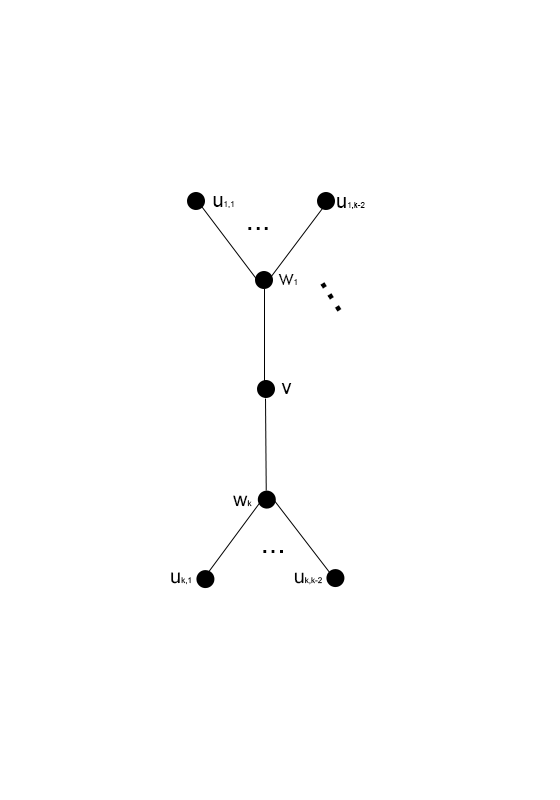
\includegraphics[width=\textwidth]{imagenes/grafos-ej3-tp3-1.png}
                \caption{}
        \end{subfigure}%
\end{figure}



 Ahora, al ordenar los nodos según su grado nos quedaría $v$ con $k$ vecinos, luego $w_i$ con $1 \leq i \leq k$, donde cada $w_i$ tiene grado $k-1$, y por último los $k * (k-2)$ nodos $u$ de grado 1. Al correr el algoritmo goloso, este arrojaría un DCIM con cardinalidad $k * (k-2) + 1$ ya que el algoritmo seleccionará a $v$ y a $u_{i,j}$ con $1 \leq i \leq k$ y $1 \leq j \leq k-2$. \\ 

\begin{figure}[H]
\centering
\begin{subfigure}[b]{0.5\textwidth}
                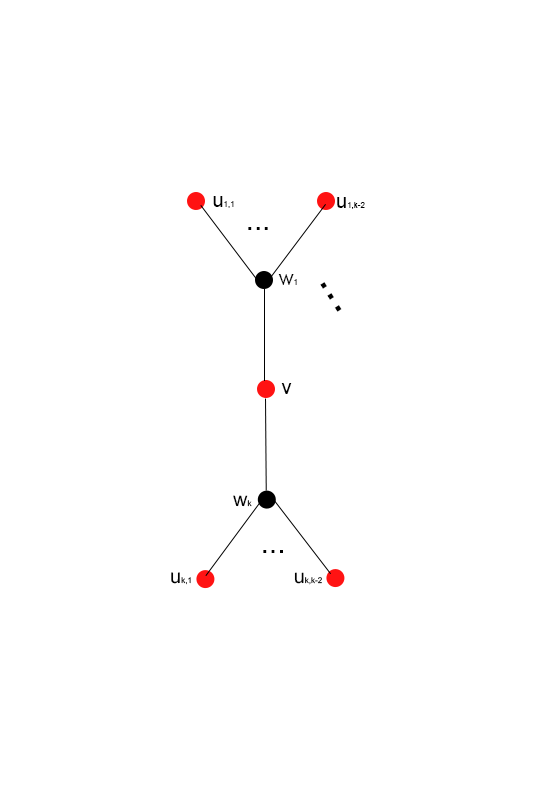
\includegraphics[width=\textwidth]{imagenes/grafos-ej3-tp3-2.png}
                \caption{}
        \end{subfigure}%
\end{figure}


 Sin embargo, si seleccionamos a todos los  $w_i$ con $1 \leq i \leq k$, tendríamos un DCIM real con cardinalidad $k$ que es mucho menor que el arrojado por el algoritmo.

\begin{figure}[H]
\centering
\begin{subfigure}[b]{0.5\textwidth}
                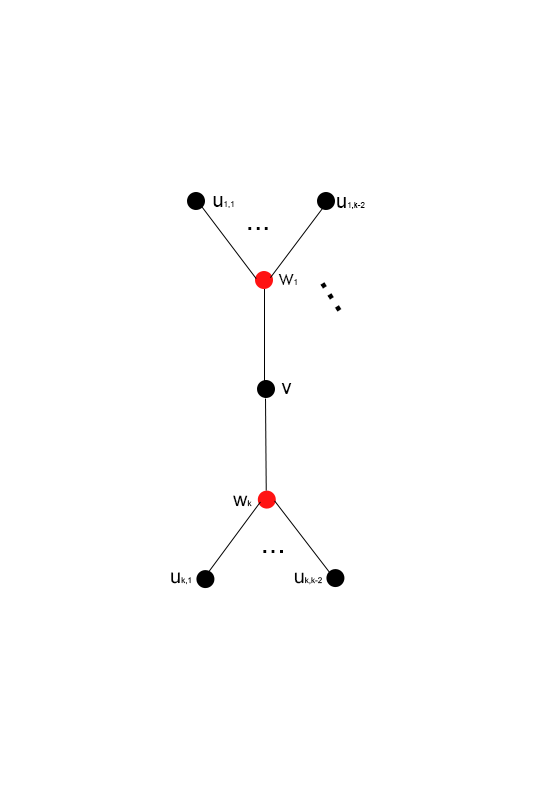
\includegraphics[width=\textwidth]{imagenes/grafos-ej3-tp3-3.png}
                \caption{}
        \end{subfigure}%
\end{figure}


Veamos que en este grafo $G=(V,E)$ tenemos $|V| = n = 1 + k*(k-1)$ por lo tanto, los $n$ para los cuales esta familia de instancias existe son los que satisfacen la ecuación con $k$ entero. Ahora, el algoritmo goloso arroja una solución de tamaño $1 + k*(k-2)$ es decir, solo quedan sin seleccionar $k$ nodos. Sin embargo, la solución optima sólo utiliza $k$ nodos.\\ 

Por lo que el error de la solución golosa es de $1 + k*(k-2) - k = 1 + k^2 -2k -k = 1 + k^2 - 3k = k^2 - 3k + 1$ que es cuadrático en el tamaño de k

\subsection{Ejercicio D}

Para la experimentación decidimos comparar distintas familias de instancias tanto en la implementación sobre matriz como el a de listas de adyacencia y comparar la eficiencia de ambas.

\subsubsection{Experimentación sobre grafo completo}

Se crearon instancias de grafos completos con $1 \leq n \leq 1000$.

En la implementación sobre matrices arrojo los siguientes resultados:\\ 

\begin{figure}[H]
        \centering
\begin{subfigure}[b]{0.5\textwidth}
                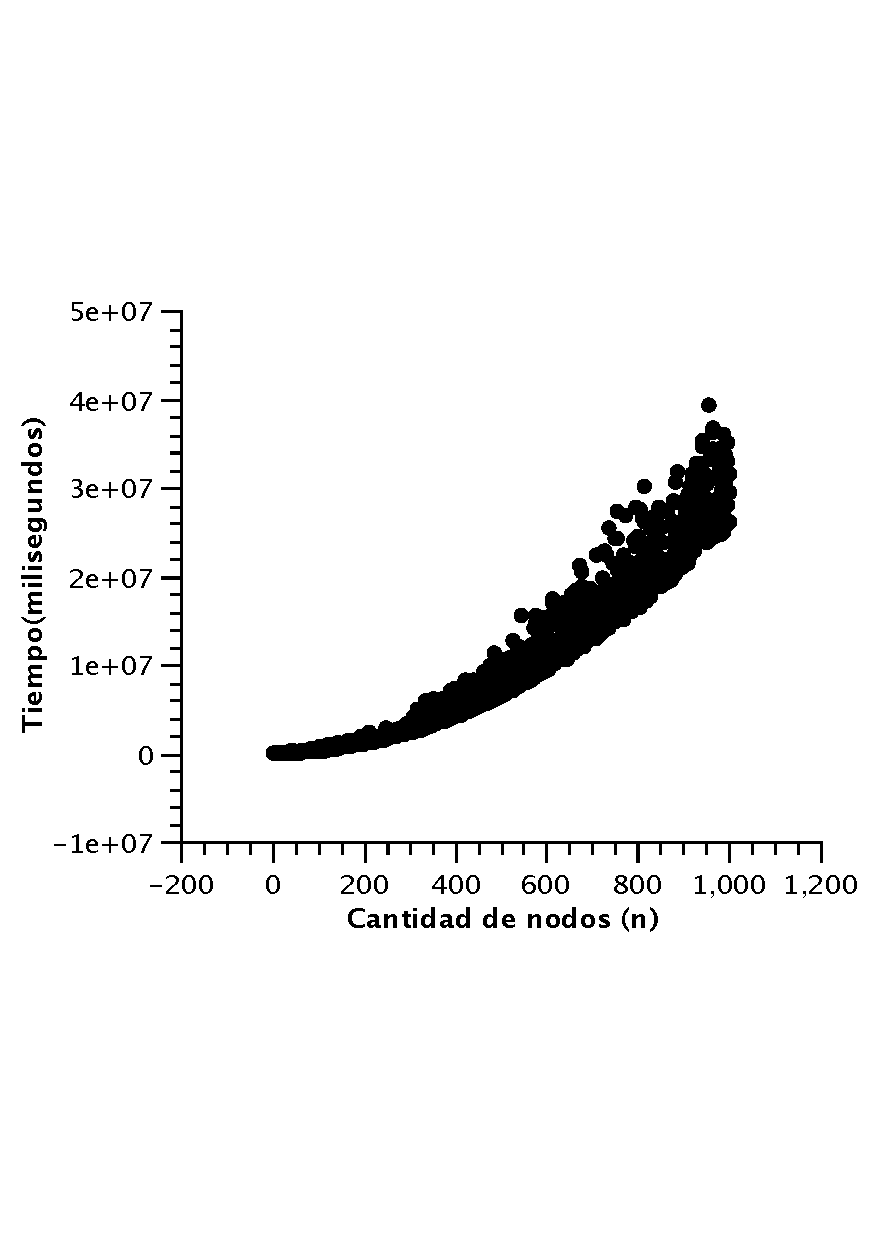
\includegraphics[width=\textwidth]{imagenes/completo-matriz-1.pdf}
                \caption{Tiempos sin procesar, en milisegundos}
        \end{subfigure}%

        \begin{subfigure}[b]{0.5\textwidth}
                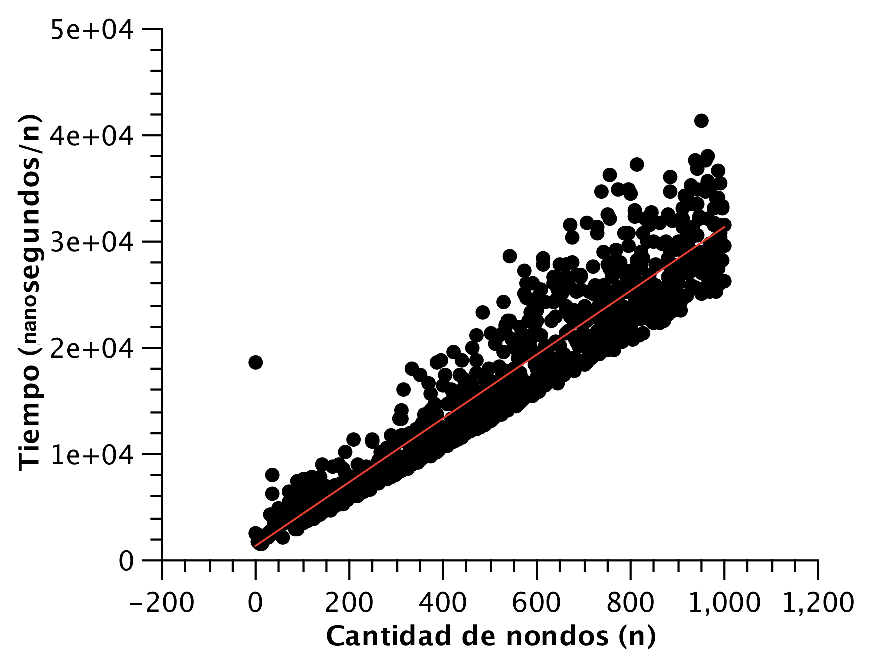
\includegraphics[width=\textwidth]{imagenes/completo-matriz-2.pdf}
                \caption{Dividiendo a los tiempos por $n$}
        \end{subfigure}

\end{figure}

\begin{figure}[H]
        \centering
        \begin{subfigure}[b]{0.5\textwidth}
                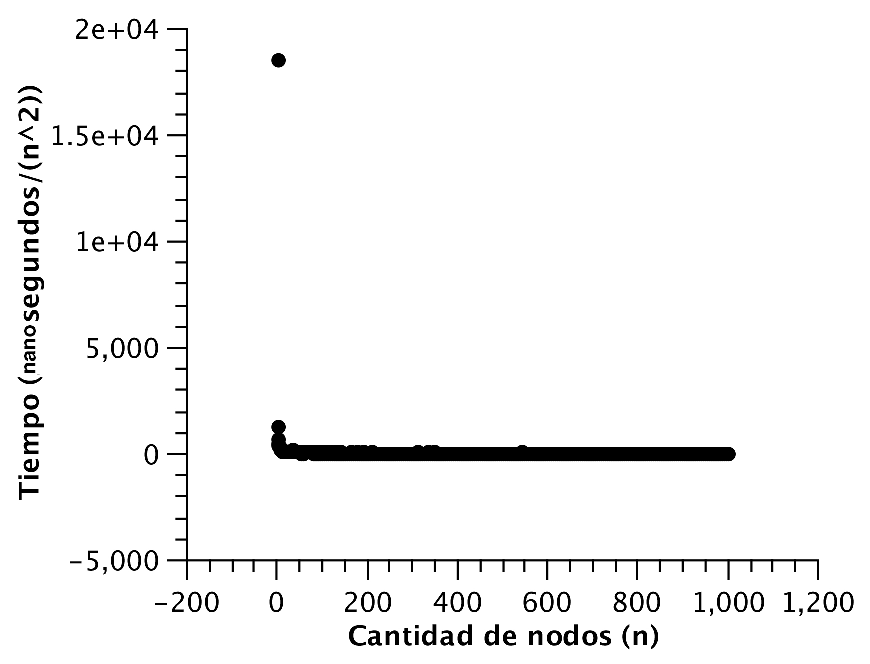
\includegraphics[width=\textwidth]{imagenes/completo-matriz-3.pdf}
                \caption{Dividiendo a los tiempos por $n^2$}
        \end{subfigure}

        \begin{subfigure}[b]{0.5\textwidth}
                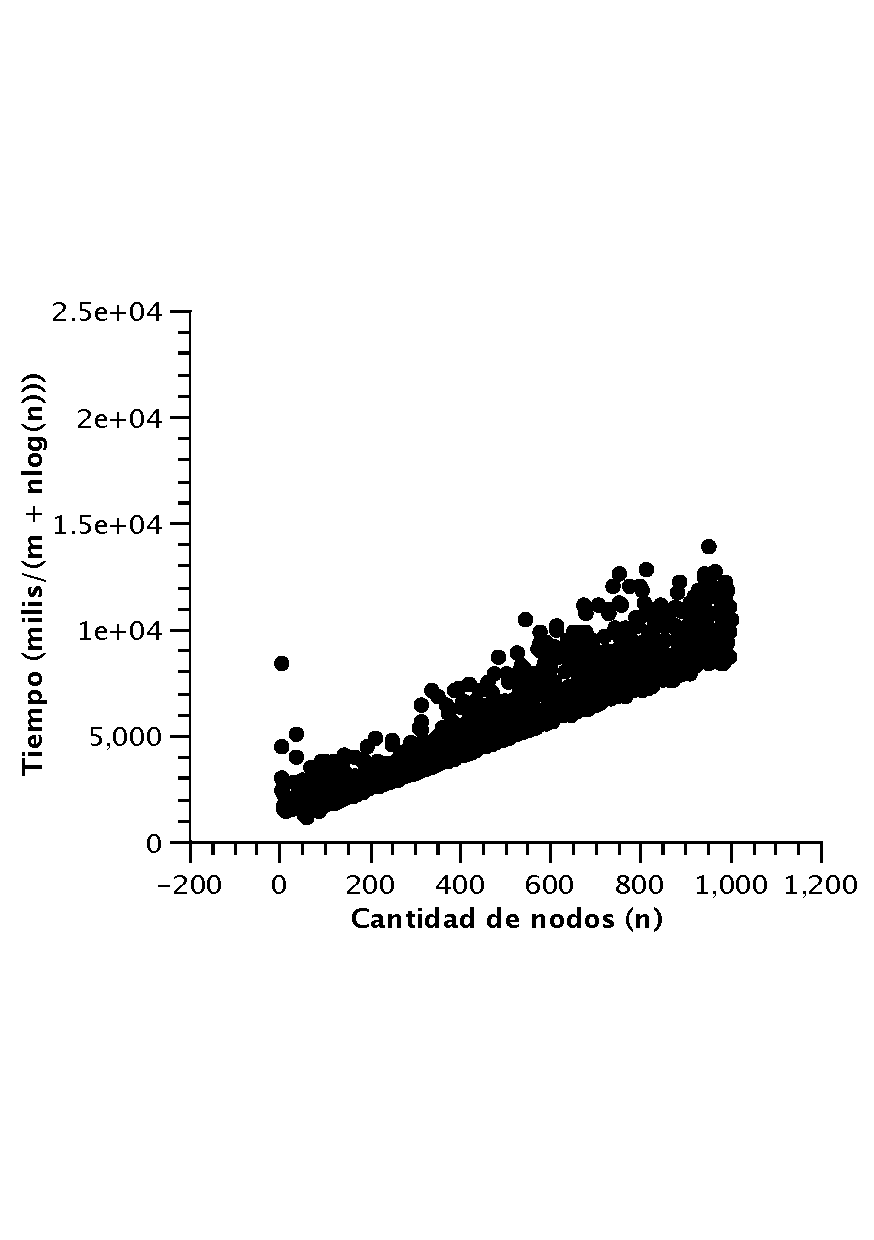
\includegraphics[width=\textwidth]{imagenes/completo-matriz-4.pdf}
                \caption{Dividiendo a los tiempos por $n + n*log(n)$}
        \end{subfigure}
\end{figure}

A continuación, adjuntamos una tabla con los últimos 20 valores obtenidos en las instancias, teniendo en cuenta que los casos fueron previamente ordenados según el tamaño ($n$):

\begin{table}[H]
\parbox{0.3\textwidth}{
    \begin{tabular}{ | l | l | l | l | l | l |}
    \hline
n   &Tiempo(milis) &m &Tiempo(mili/($n$)) &Tiempo(mili/($n^2$))) &Tiempo(mili/($n*log(n) + m$)))\\ \hline
980	&24,845,670	&479710	&25,352.72448979592	&25.870127030404	&8,475.696536553674\\ \hline
981	&33,412,818	&480690	&34,059.95718654434	&34.71963015957629	&11,384.934998666\\ \hline
982	&24,857,309	&481671	&25,312.94195519348	&25.77692663461658	&8,459.892640536484\\ \hline
983	&29,750,650	&482653	&30,265.15768056969	&30.78856325592033	&10,113.4891991821\\ \hline
984	&25,165,002	&483636	&25,574.18902439025	&25.99002949633155	&8,544.681225102551\\ \hline
985	&28,427,751	&484620	&28,860.66091370558	&29.3001633641681	&9,641.314760497822\\ \hline
986	&27,111,085	&485605	&27,496.02941176471	&27.88643956568429	&9,184.088121506702\\ \hline
987	&36,119,756	&486591	&36,595.49746707194	&37.07750503249436	&12,221.65041349897\\ \hline
988	&33,731,556	&487578	&34,141.25101214575	&34.5559220770706	&11,400.34121094489\\ \hline
989	&30,542,586	&488566	&30,882.29120323559	&31.22577472521294	&10,310.60678389385\\ \hline
990	&31,176,002	&489555	&31,490.91111111111	&31.80900112233446	&10,512.26503410799\\ \hline
991	&30,168,178	&490545	&30,442.15741675076	&30.71862504212993	&10,160.68392416765\\ \hline
992	&25,911,896	&491536	&26,120.86290322581	&26.33151502341311	&8,717.090324045907\\ \hline
993	&35,168,815	&492528	&35,416.73212487412	&35.6663969031965	&11,817.59489008868\\ \hline
994	&28,113,874	&493521	&28,283.5754527163	&28.45430126027797	&9,436.079245553556\\ \hline
995	&33,158,039	&494515	&33,324.66231155779	&33.49212292618873	&11,116.28719039287\\ \hline
996	&26,079,861	&495510	&26,184.59939759036	&26.28975843131563	&8,733.26701997587\\ \hline
997	&33,013,519	&496506	&33,112.85757271815	&33.21249505789183	&11,042.42206178822\\ \hline
998 &29,605,093	&497503	&29,664.42184368737	&29.72386958285308	&9,891.007222031083\\ \hline
999	&26,197,019	&498501	&26,223.24224224224	&26.24949173397622	&8,742.346964977023\\ \hline
1,000	&31,613,146	&499500	&31,613.146	&31.613146	&10,537.71533333333\\ \hline
    \end{tabular}
}
\end{table}

Como podemos ver la experimentación se condice con el cálculo teórico de la complejidad y arroja que es de $\mathcal{O}(n^2)$.

Veamos ahora los resultados en la implementación sobre listas de adyacencia:

\begin{figure}[H]
        \centering
\begin{subfigure}[b]{0.5\textwidth}
                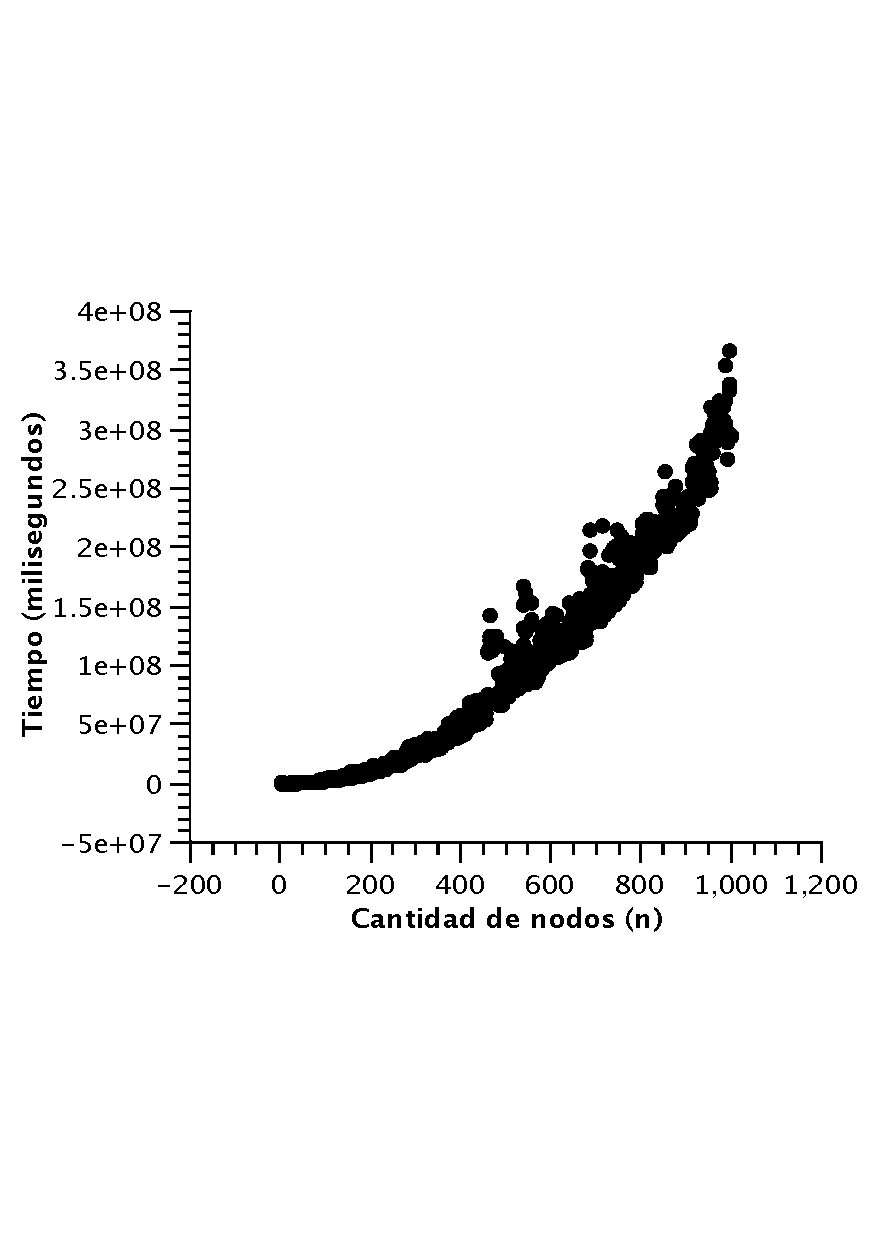
\includegraphics[width=\textwidth]{imagenes/completo-listas-1.pdf}
                \caption{Tiempos sin procesar, en milisegundos}
        \end{subfigure}%

        \begin{subfigure}[b]{0.5\textwidth}
                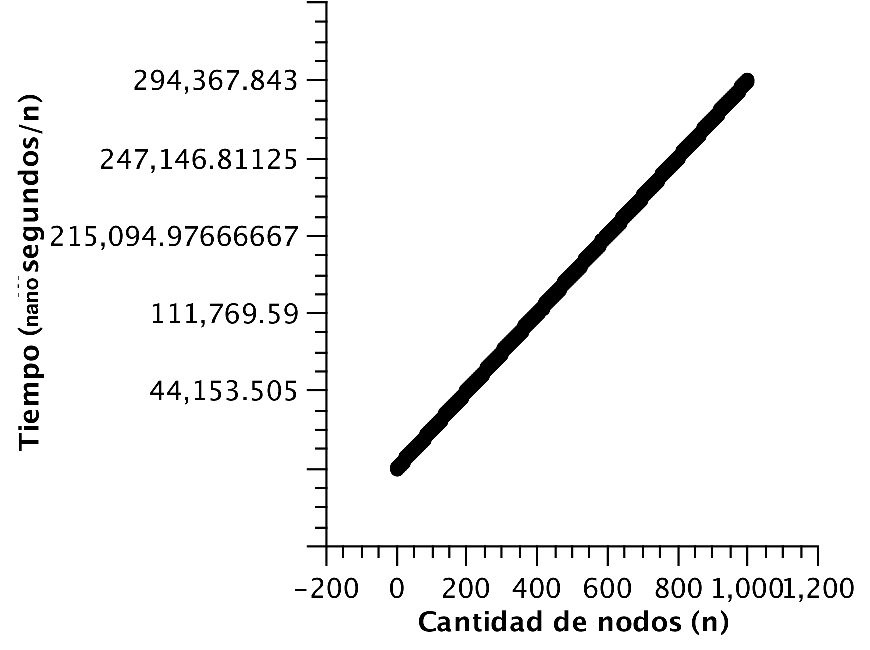
\includegraphics[width=\textwidth]{imagenes/completo-listas-2.pdf}
                \caption{Dividiendo a los tiempos por $n$}
        \end{subfigure}
\end{figure}

\begin{figure}[H]
        \centering
         \begin{subfigure}[b]{0.5\textwidth}
                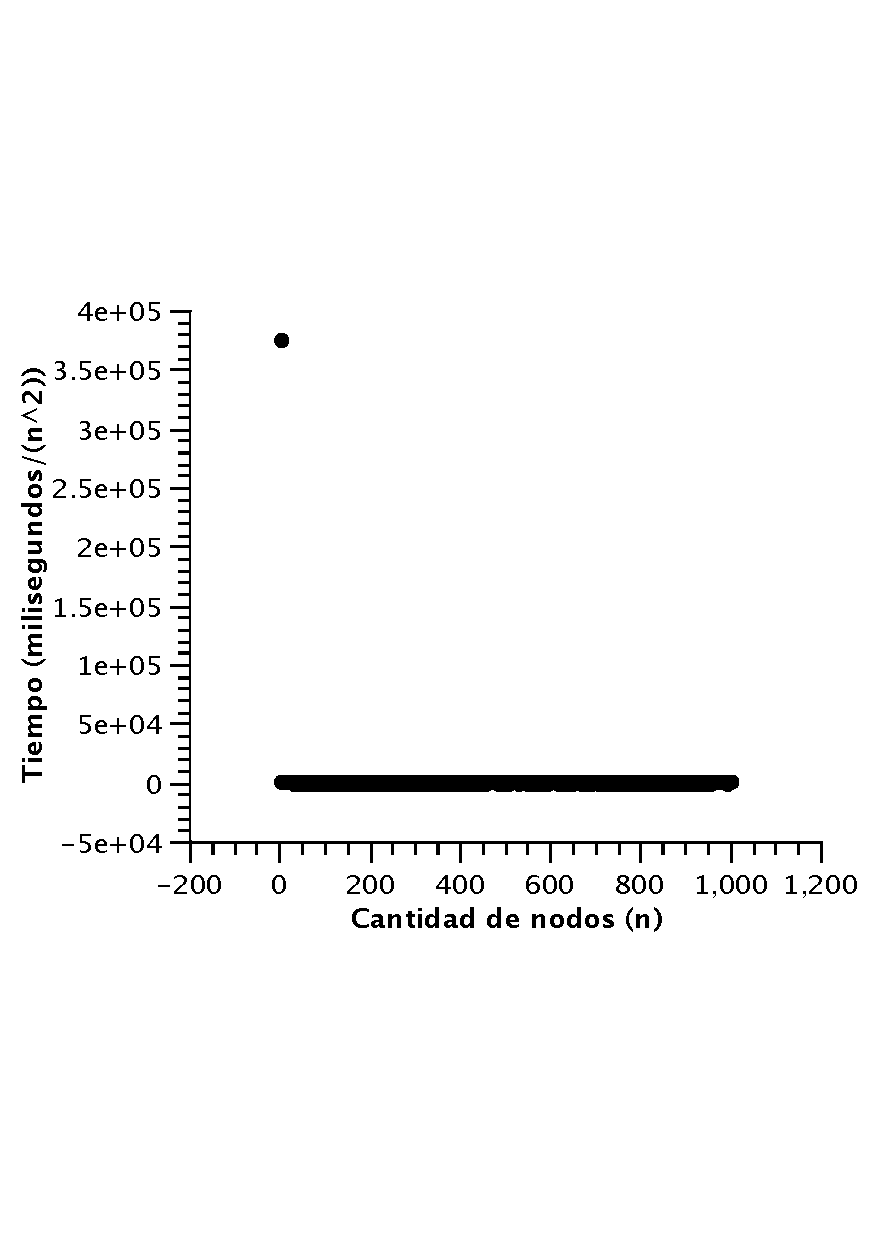
\includegraphics[width=\textwidth]{imagenes/completo-listas-3.pdf}
                \caption{Dividiendo a los tiempos por $n^2$}
        \end{subfigure}

        \begin{subfigure}[b]{0.5\textwidth}
                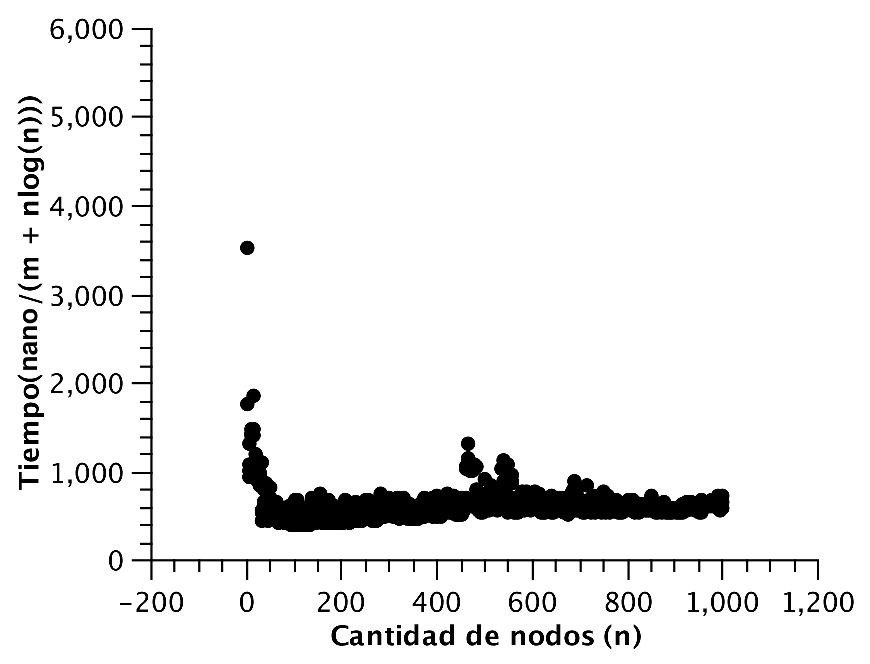
\includegraphics[width=\textwidth]{imagenes/completo-listas-4.pdf}
                \caption{Dividiendo a los tiempos por $n + n*log(n)$}
        \end{subfigure}
\end{figure}
A continuación, adjuntamos una tabla con los últimos 20 valores obtenidos en las instancias, teniendo en cuenta que los casos fueron previamente ordenados según el tamaño ($n$):

\begin{table}[H]
\parbox{0.3\textwidth}{
    \begin{tabular}{ | l | l | l | l | l | l |}
    \hline
n   &Tiempo(milis) &Tiempo(mili/($n$)) &Tiempo(mili/($n^2$))) &Tiempo(mili/($n*log(n) + m$))) &m\\ \hline
980	&296,879,716	&302,938.48571429	&309.1209037900875	&615.1144826034448	&479,710\\ \hline
981	&323,033,524	&329,290.03465851	&335.667721364436	&667.9423920520295	&480,690\\ \hline
982	&292,431,614	&297,791.86761711	&303.2503743555071	&603.4379490268261	&481,671\\ \hline
983	&297,273,430	&302,414.47609359	&307.6444314278647	&612.1842807953875	&482,653\\ \hline
984	&318,286,205	&323,461.59044715	&328.7211285032058	&654.1277503491588	&483,636\\ \hline
985	&308,937,975	&313,642.6142132	&318.4188976783736	&633.6298448756557	&484,620\\ \hline
986	&323,384,902	&327,976.57403651	&332.6334422276989	&661.9185207263685	&485,605\\ \hline
987	&304,973,689	&308,990.56636272	&313.0603509247369	&622.9719891480256	&486,591\\ \hline
988	&302,281,783	&305,953.22165992	&309.6692526922257	&616.2264905731232	&487,578\\ \hline
989	&353,599,216	&357,532.06875632	&361.5086640609904	&719.3873732062154	&488,566\\ \hline
990	&292,805,769	&295,763.4030303	&298.7509121518212	&594.5045184459034	&489,555\\ \hline
991	&289,577,857	&292,207.72653885	&294.8614798575678	&586.7671292958553	&490,545\\ \hline
992	&289,158,638	&291,490.5625	    &293.841292842742	&584.7394227940042	&491,536\\ \hline
993	&293,229,428	&295,296.50352467	&297.3781505787238	&591.7801781541916	&492,528\\ \hline
994	&275,111,868	&276,772.50301811	&278.443161990049	&554.102004459966	&493,521\\ \hline
995	&333,606,954	&335,283.37085427	&336.9682119138405	&670.5696612605566	&494,515\\ \hline
996	&338,319,005	&339,677.71586345	&341.041883397042	&678.679115312912	&495,510\\ \hline
997	&332,699,588	&333,700.69007021	&334.7048044836616	&666.0709764219323	&496,506\\ \hline
998	&366,440,239	&367,174.58817635	&367.9104089943414	&732.1539875453961	&497,503\\ \hline
999	&296,662,430	&296,959.38938939	&297.2566460354248	&591.5530805302149	&498,501\\ \hline
1,000	&294,367,843	&294,367.843    &294.367843         &585.8066527363184  &499,500\\ \hline
    \end{tabular}
}
\end{table}

Como podemos ver, la experimentación se condice con el cálculo teórico de la complejidad y arroja que es de $\mathcal{O}(n*log(n) + m)$, aunque en un grafo completo es casi $\mathcal{O}(n^2)$.



\subsubsection{Experimentación sobre el complemento del grafo completo}

Se crearon instancias de complementos grafos completos con $1 \leq n \leq 1000$ y $m = 0$.

En la implementación sobre matrices arrojo los siguientes resultados:\\ 

\begin{figure}[H]
        \centering
\begin{subfigure}[b]{0.5\textwidth}
                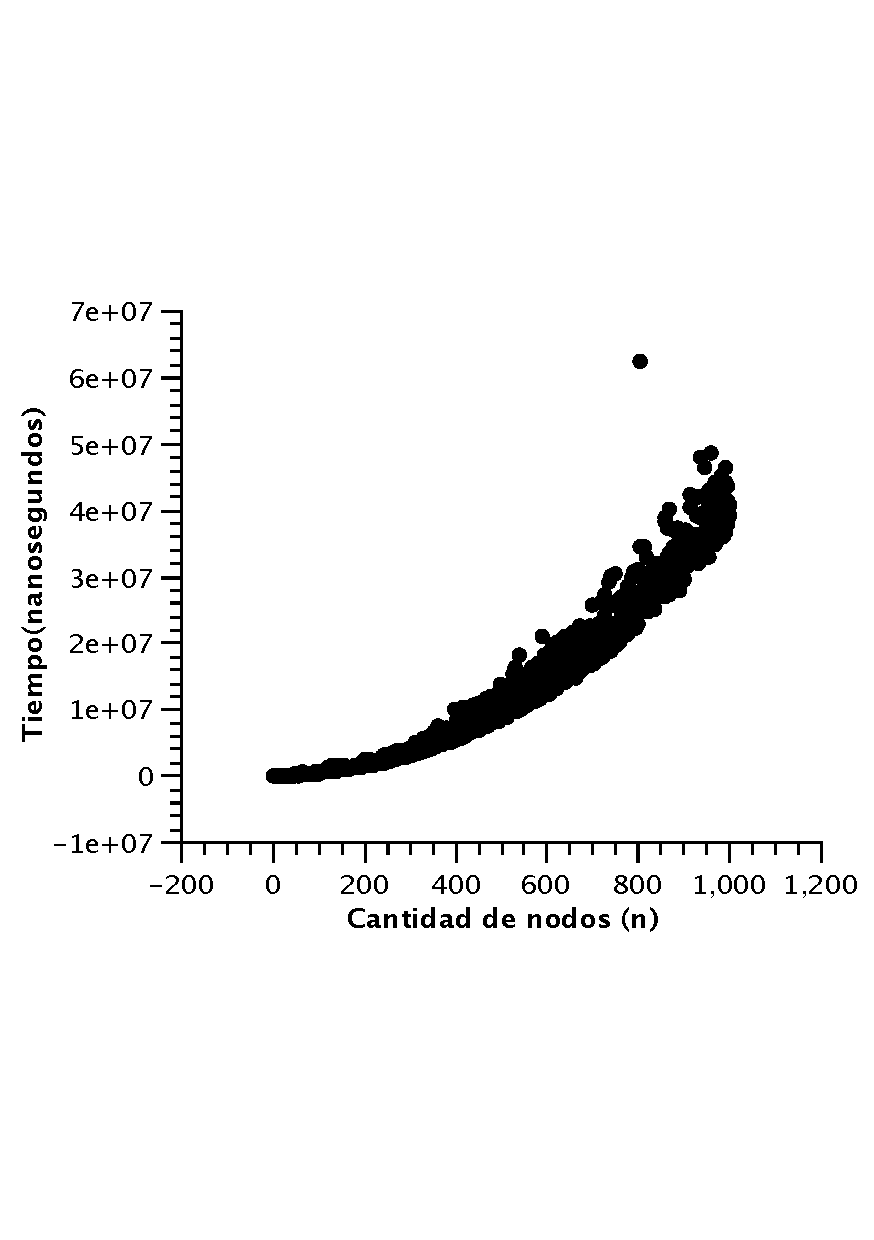
\includegraphics[width=\textwidth]{imagenes/vacio-matriz-1.pdf}
                \caption{Tiempos sin procesar, en milisegundos}
        \end{subfigure}%

        \begin{subfigure}[b]{0.5\textwidth}
                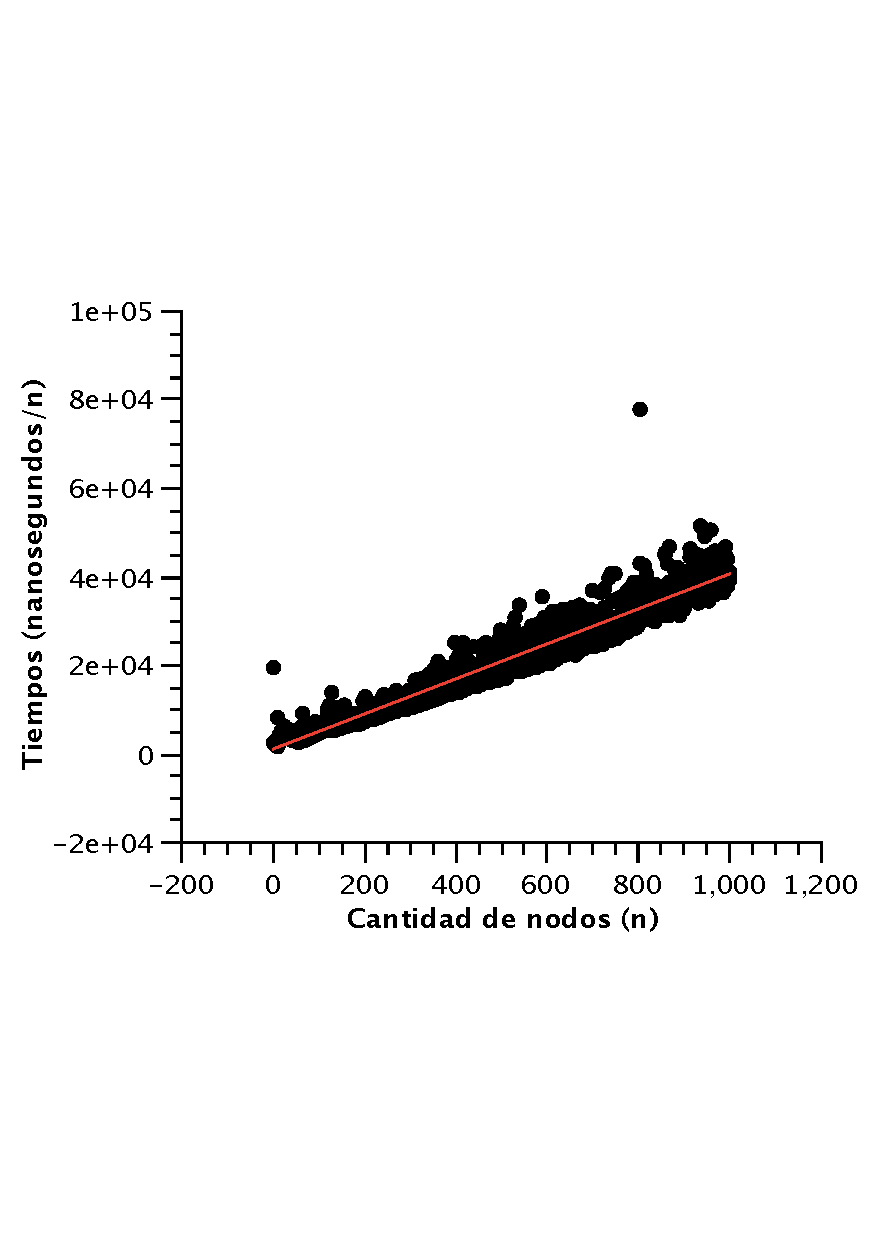
\includegraphics[width=\textwidth]{imagenes/vacio-matriz-2.pdf}
                \caption{Dividiendo a los tiempos por $n$}
        \end{subfigure}



\end{figure}

\begin{figure}[H]
        \centering
        \begin{subfigure}[b]{0.5\textwidth}
                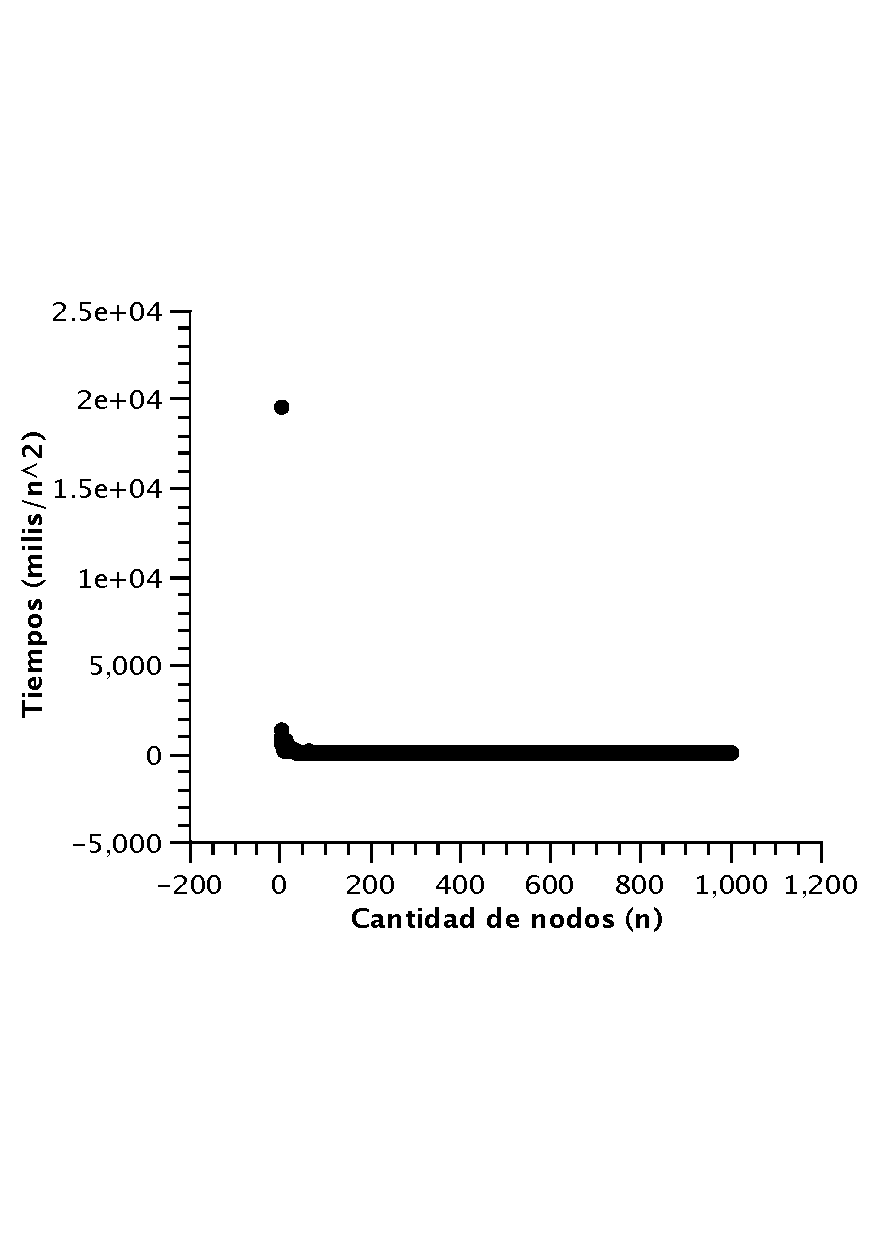
\includegraphics[width=\textwidth]{imagenes/vacio-matriz-3.pdf}
                \caption{Dividiendo a los tiempos por $n^2$}
        \end{subfigure}

        \begin{subfigure}[b]{0.5\textwidth}
                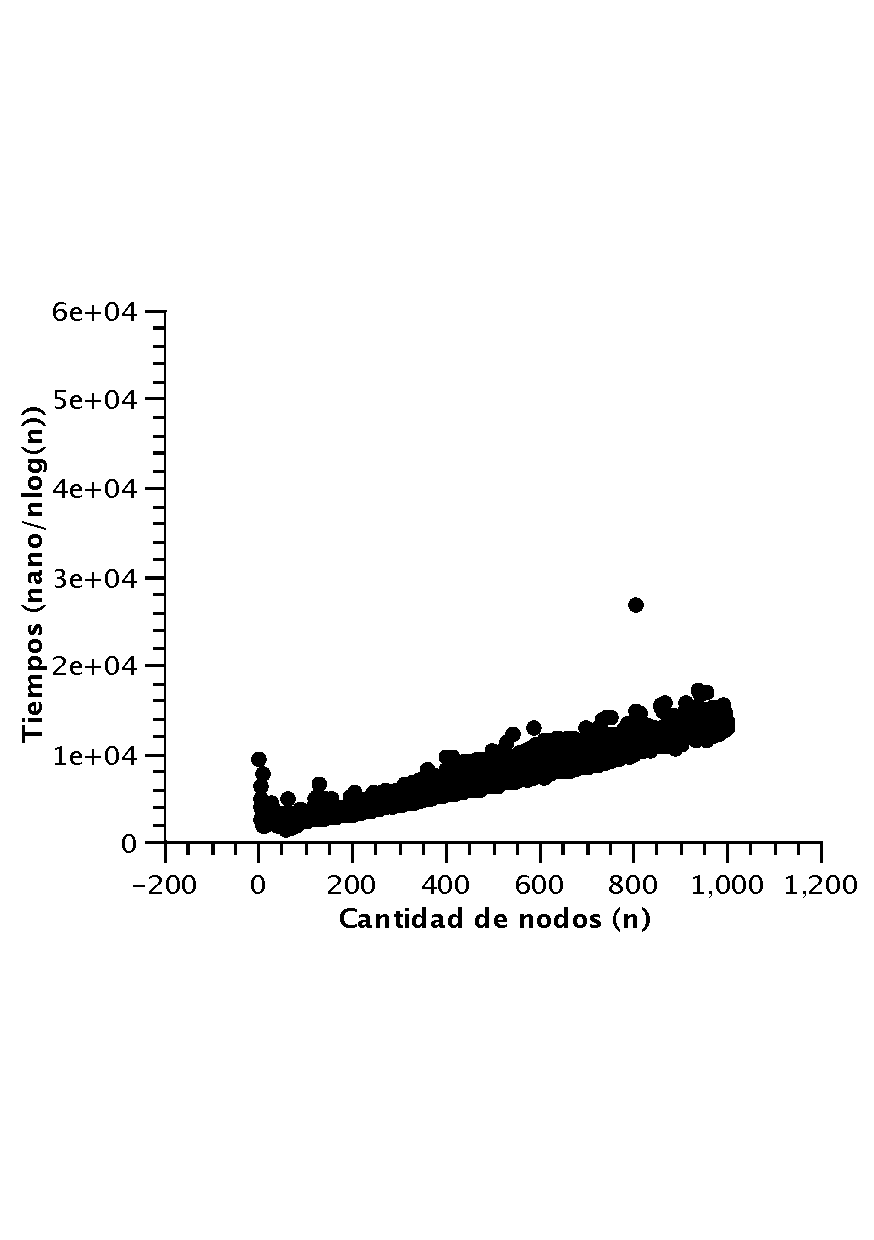
\includegraphics[width=\textwidth]{imagenes/vacio-matriz-4.pdf}
                \caption{Dividiendo a los tiempos por $n + n*log(n)$}
        \end{subfigure}
\end{figure}

A continuación, adjuntamos una tabla con los últimos 20 valores obtenidos en las instancias, teniendo en cuenta que los casos fueron previamente ordenados según el tamaño ($n$):

\begin{table}[H]
\parbox{0.3\textwidth}{
    \begin{tabular}{ | l | l | l | l | l |}
    \hline
n   &Tiempo(milis) &Tiempo(mili/($n$)) &Tiempo(mili/($n^2$))) &Tiempo(mili/($n*log(n) + m$)))\\ \hline
980	&41,753,937	&42,606.0581632653	&43.47556955435235	&14,243.67703581269\\ \hline
981	&37,549,011	&38,276.25993883792	&39.01759422919258	&12,794.28300537819\\ \hline
982	&39,391,112	&40,113.14867617108	&40.84842024050008	&13,406.30148305065\\ \hline
983	&45,239,903	&46,022.28179043744	&46.81819103808488	&15,378.93358170479\\ \hline
984	&36,000,279	&36,585.6493902439	&37.18053799821535	&12,223.75853853513\\ \hline
985	&43,702,767	&44,368.29137055838	&45.0439506300085	&14,821.85954673998\\ \hline
986	&40,825,343	&41,405.01318458418	&41.99291398030849	&13,829.89827602756\\ \hline
987	&38,862,643	&39,374.5116514691	&39.89312224059685	&13,149.74655118415\\ \hline
988	&36,831,350	&37,278.6943319838	&37.73147199593502	&12,447.98660517573\\ \hline
989	&44,397,040	&44,890.83923154702	&45.39013066890497	&14,987.61178273532\\ \hline
990	&39,102,722	&39,497.69898989899	&39.89666564636262	&13,185.08310395429\\ \hline
991	&40,118,814	&40,483.16246215944	&40.85081984072598	&13,512.07184160979\\ \hline
992	&46,471,583	&46,846.35383064516	&47.22414700669875	&15,633.62968546942\\ \hline
993	&41,389,046	&41,680.81168177241	&41.97463412061673	&13,907.7469205387\\ \hline
994	&43,743,891	&44,007.93863179074	&44.27358011246553	&14,682.10400263076\\ \hline
995	&38,823,308	&39,018.4	        &39.21447236180904	&13,015.57795408459\\ \hline
996	&37,960,325	&38,112.77610441767	&38.26583946226674	&12,711.63425257771\\ \hline
997	&39,036,157	&39,153.61785356068	&39.27143215001071	&13,056.88500714597\\ \hline
998	&40,876,628	&40,958.54509018036	&41.0406263428661	&13,656.80637315606\\ \hline
999	&40,732,820	&40,773.59359359359	&40.81440800159519	&13,593.16666151807\\ \hline
    \end{tabular}
}
\end{table}

Como podemos ver, la experimentación se condice con el cálculo teórico de la complejidad y, aunque el no haya aristas en el grafo, la complejidad que arroja es de $\mathcal{O}(n^2)$.


Veamos ahora los resultados en la implementación sobre listas de adyacencia:

\begin{figure}[H]
        \centering
\begin{subfigure}[b]{0.5\textwidth}
                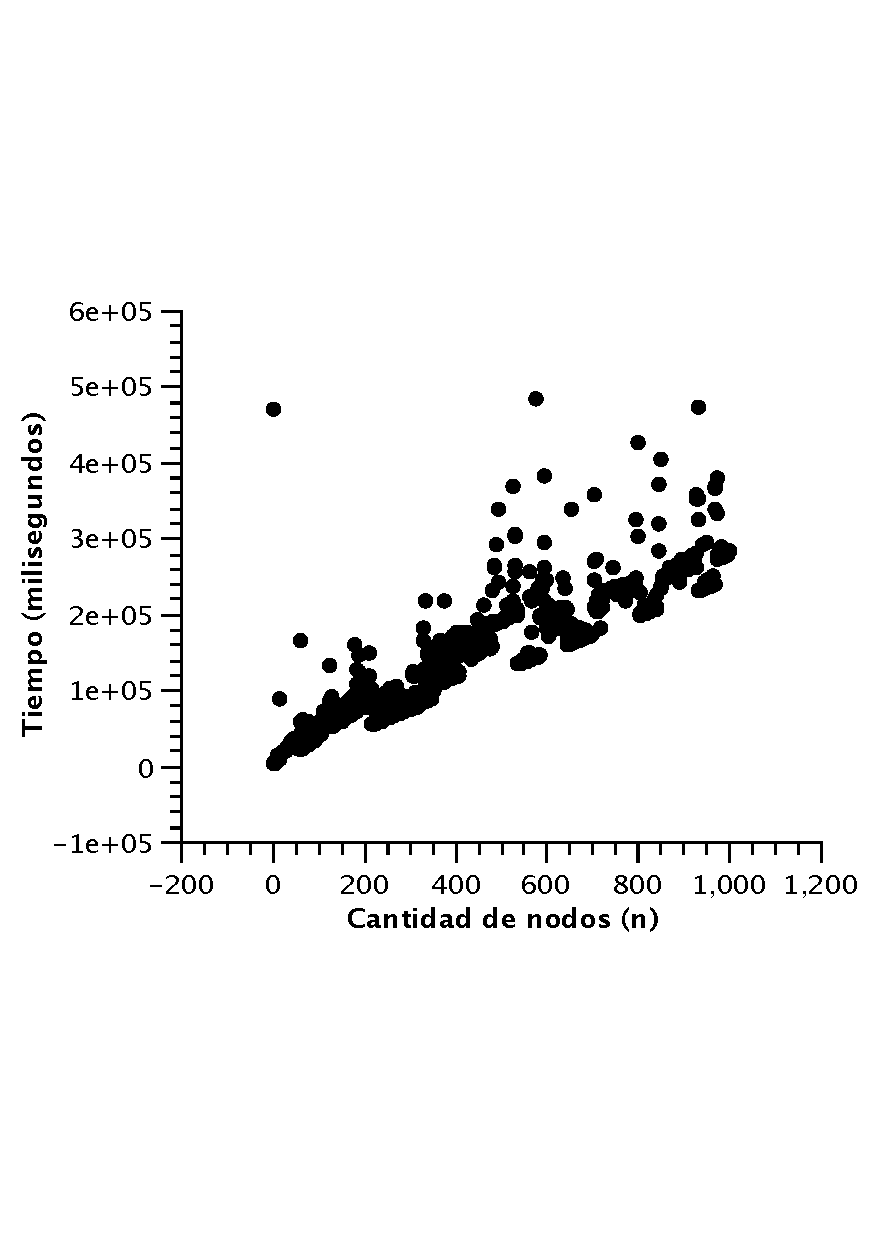
\includegraphics[width=\textwidth]{imagenes/vacio-listas-1.pdf}
                \caption{Tiempos sin procesar, en milisegundos}
        \end{subfigure}%

        \begin{subfigure}[b]{0.5\textwidth}
                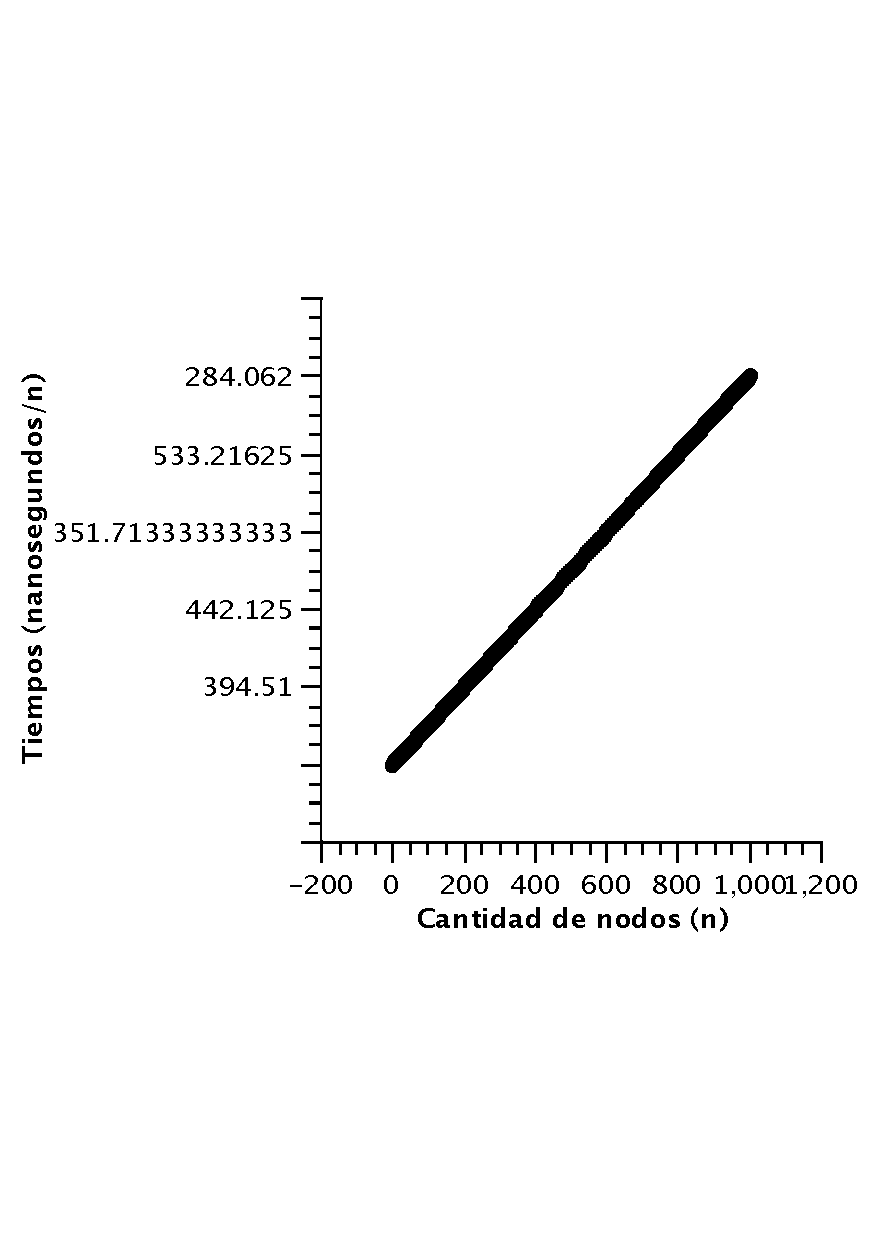
\includegraphics[width=\textwidth]{imagenes/vacio-listas-2.pdf}
                \caption{Dividiendo a los tiempos por $n$}
        \end{subfigure}


\end{figure}

\begin{figure}[H]
        \centering
        \begin{subfigure}[b]{0.5\textwidth}
                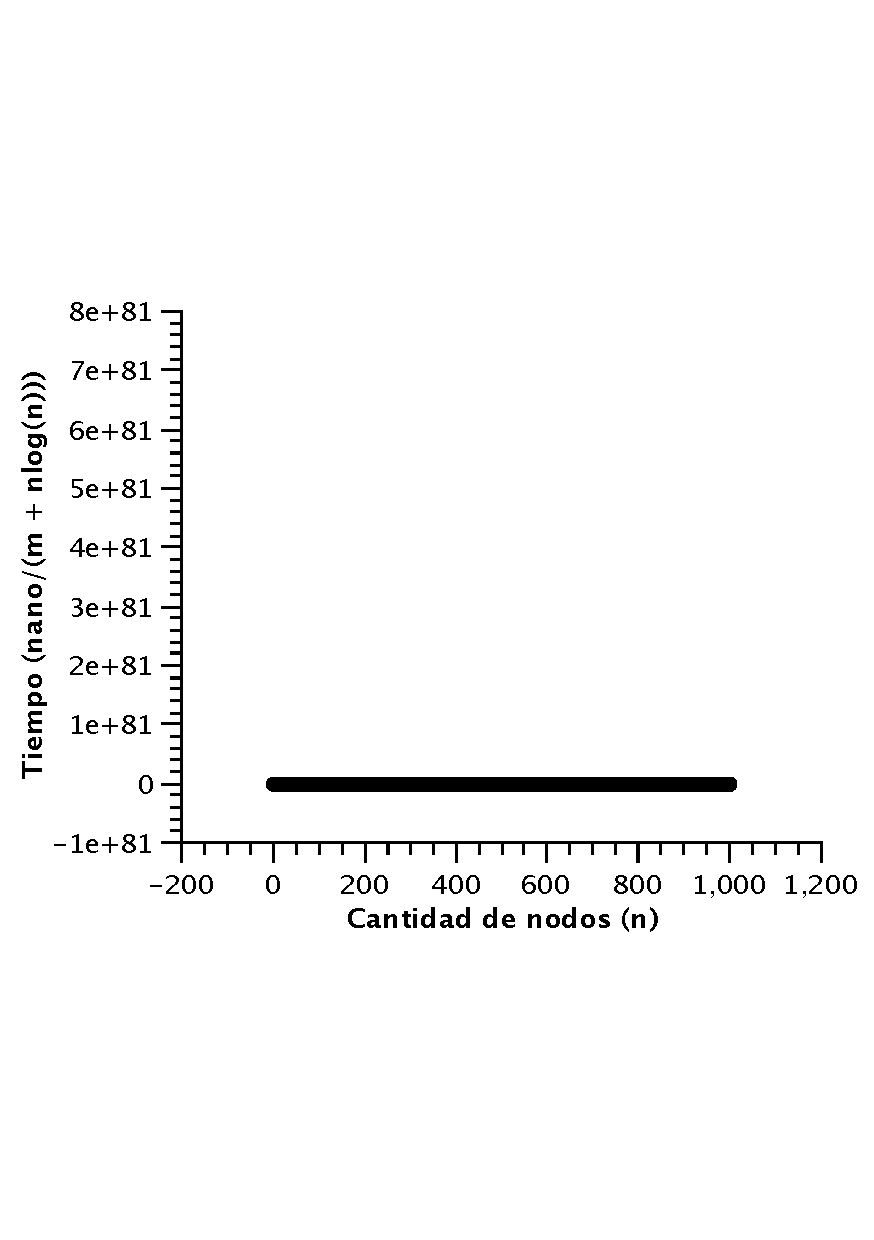
\includegraphics[width=\textwidth]{imagenes/vacio-listas-3.pdf}
                \caption{Dividiendo a los tiempos por $n^2$}
        \end{subfigure}

        \begin{subfigure}[b]{0.5\textwidth}
                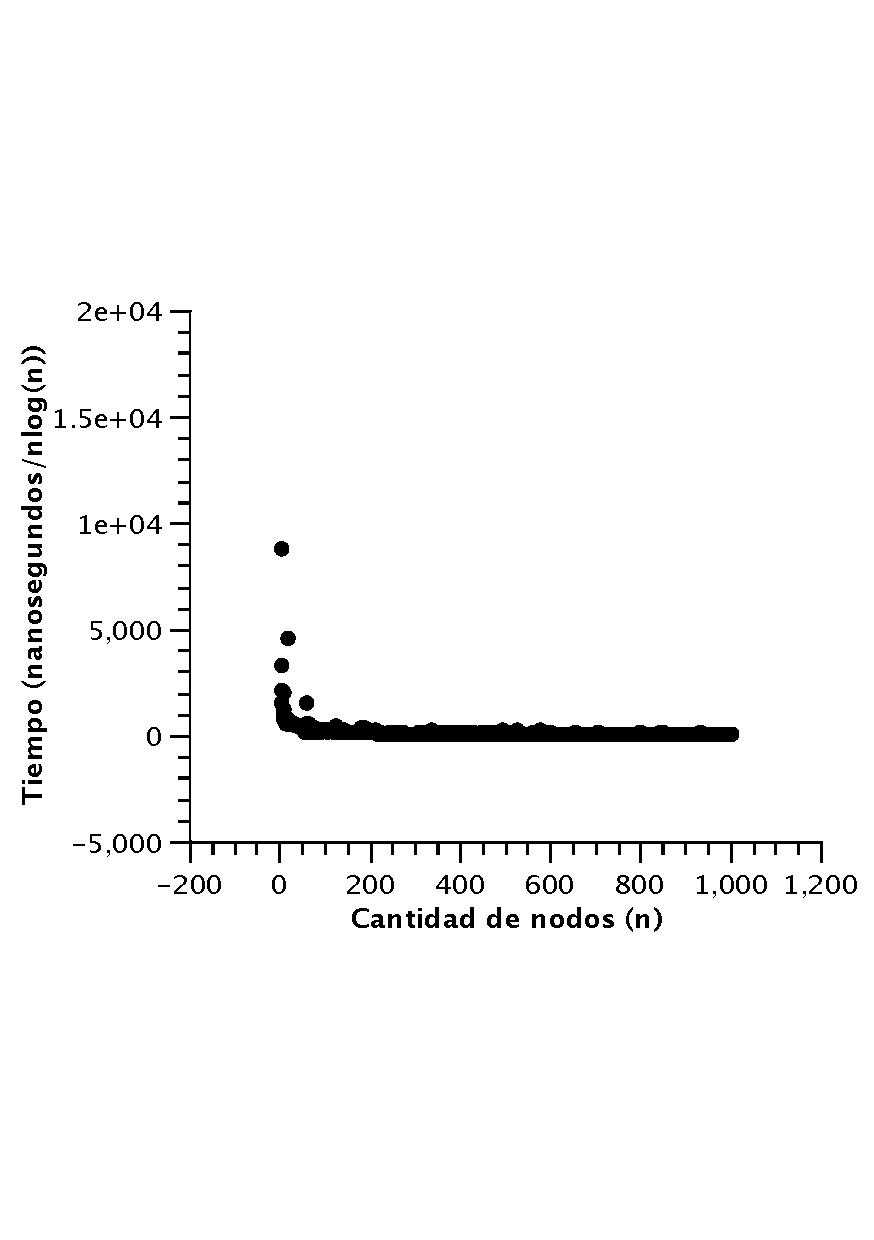
\includegraphics[width=\textwidth]{imagenes/vacio-listas-4.pdf}
                \caption{Dividiendo a los tiempos por $n + n*log(n)$}
        \end{subfigure}

\end{figure}

A continuación, adjuntamos una tabla con los últimos 20 valores obtenidos en las instancias, teniendo en cuenta que los casos fueron previamente ordenados según el tamaño ($n$):

\begin{table}[H]
\parbox{0.3\textwidth}{
    \begin{tabular}{ | l | l | l | l | l |}
    \hline
n   &Tiempo(milis) &Tiempo(mili/($n$)) &Tiempo(mili/($n^2$))) &Tiempo(mili/($n*log(n) + m$)))\\ \hline
980	&283,093	&288.87040816327	&0.2947657226155768	&96.57257621237783\\ \hline
981	&279,943	&285.36493374108	&0.2908918794506428	&95.38653274714977\\ \hline
982	&280,415	&285.5549898167	    &0.290789195332689	&95.43594581360509\\ \hline
983	&288,893	&293.88911495422	&0.2989716327102968	&98.20680338813817\\ \hline
984	&276,797	&281.29776422764	&0.2858717116134576	&93.98537417420873\\ \hline
985	&277,190	&281.41116751269	&0.2856966167641526	&94.00940786565884\\ \hline
986	&276,617	&280.54462474645	&0.2845280169842295	&93.70613178730468\\ \hline
987	&277,663	&281.3201621074	    &0.2850254935231977	&93.95135777670718\\ \hline
988	&281,872	&285.2955465587	    &0.2887606746545592	&95.26500875949687\\ \hline
989	&282,107	&285.24469160768	&0.2884172817064555	&95.23405608103857\\ \hline
990	&277,617	&280.42121212121	&0.283253749617386	&93.60993375526336\\ \hline
991	&278,533	&281.06256306761	&0.2836150989582326	&93.81029823710891\\ \hline
992	&278,372	&280.61693548387	&0.2828799752861603	&93.64786998548107\\ \hline
993	&278,950	&280.91641490433	&0.2828966917465562	&93.73412480887504\\ \hline
994	&279,345	&281.03118712274	&0.2827275524373606	&93.75874548093792\\ \hline
995	&279,336	&280.73969849246	&0.2821504507461933	&93.64785410306024\\ \hline
996	&278,955	&280.07530120482	&0.2812001016112644	&93.41263366232546\\ \hline
997	&283,107	&283.95887662989	&0.2848133165796286	&94.69414583300491\\ \hline
998	&283,434	&284.00200400802	&0.2845711463006173	&94.69477906957285\\ \hline
999	&283,640	&283.92392392392	&0.2842081320559799	&94.65501754783944\\ \hline
1,000	&284,062	&284.062	&0.284062	&94.68733333333333\\ \hline
    \end{tabular}
}
\end{table}

Como podemos ver, la experimentación se condice con el cálculo teórico de la complejidad y arroja que es de $\mathcal{O}(n*log(n) + m)$, sin embargo, como el grafo no tiene aristas, aqui la complejidad es de $\mathcal{O}(n*log(n))$ siendo así más eficiente que en la implementación sobre matriz de adyacencia.







